%------------------------------------------------------------------------
%Editar Diplomado
\hypertarget{cv:modificarPExt}{\section{Modificar Punto de Extensión}} \label{sec:modificarPExt}

	Esta funcionalidad le permitirá modificar la información de un punto de extensión previamente registrado con el fin de corregir o actualizar datos del mismo. 

		\subsection{Procedimiento}

			%Pasos de procedimiento
			\begin{enumerate}
	
			\item Oprima el botón \IUEditar{} de algún registro existente de la pantalla \ref{fig:GestionarPuntosExt} ''Gestionar Puntos de Extensión''.
	
			\item Se mostrará la pantalla \ref{fig:modificarPExt} ''Modificar Punto de Extensión''.
			
			%Pantalla
			\begin{figure}[htbp!]
				\begin{center}
					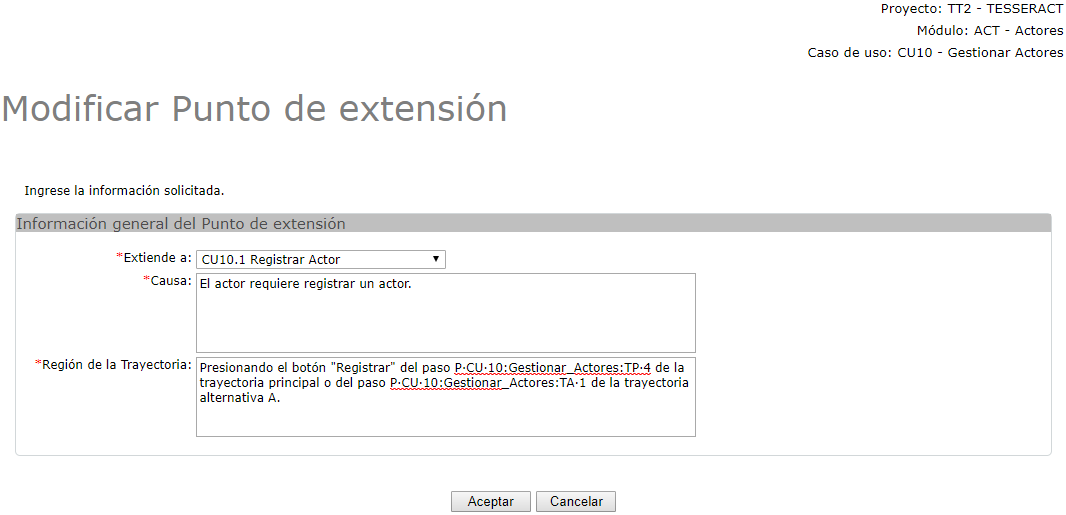
\includegraphics[scale=0.5]{roles/lider/puntosExtension/pantallas/IU6-1-4-2modificarPuntosExt}
					\caption{Modificar Punto de Extensión}
					\label{fig:modificarPExt}
				\end{center}
			\end{figure}
		
			\item Modifique los datos solicitados por la pantalla.
			
			\item En la región de la trayectoria usted podrá referenciar algunos tipos de elementos que se encuentren registrados dentro del proyecto actual, mendiante el siguiente TOKEN: \\Podrá referenciar elementos de tipo paso con el TOKEN: ''P·''.
						
			\item Oprima el botón \IUAceptar.
			
			\item Se mostrará el mensaje \ref{fig:pextModificada} en la pantalla \ref{fig:GestionarPuntosExt} ''Gestionar Puntos de Extensión''.
			
			\begin{figure}[htbp!]
				\begin{center}
					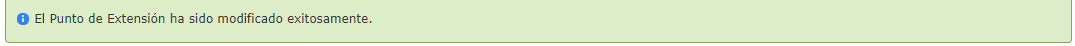
\includegraphics[scale=0.5]{roles/lider/puntosExtension/pantallas/IU6-1-4-2MSG1}
					\caption{MSG: Punto de Extensión Actualizado}
					\label{fig:pextModificada}
				\end{center}
			\end{figure}
			\end{enumerate}